\documentclass[11pt]{ltjsarticle}
\usepackage{amsmath}
\usepackage{amssymb}
\usepackage{amsfonts}
\usepackage{physics}
\usepackage{graphicx}
\usepackage{float}
\usepackage{booktabs}
\usepackage{tikz}
\usepackage{xcolor}
\usepackage{pgfplots}
\usepackage{mathcomp}
\usepackage{enumitem}
\usepackage{wrapfig}
\usepackage{etoolbox}
\usepackage{cleveref}
\usepackage[version=4]{mhchem}
\crefformat{figure}{図~#2#1#3}  % 図の日本語設定
\crefformat{equation}{式~(#2#1#3)}  % 式の日本語設定
\crefformat{table}{表~#2#1#3}  % 表の日本語設定
\usetikzlibrary{intersections,calc}
\pgfplotsset{compat=1.18}
\begin{document}
  \section*{目的}
    高温超伝導体である$\ce{YBa2Cu3O_{7-\sigma}}$を作成して, 電気抵抗, 磁化率, の温度依存性を測定する.\\
    実験を通して, 以下の四項目を学ぶ.
    \begin{enumerate}
      \item 固体反応法による試料作成
      \item 四端子法, 二端子法による電気抵抗測定
      \item 熱電対による温度測定や液体窒素の扱い方
      \item マイスナー効果の概念
    \end{enumerate}
  \section*{原理}
    \subsection*{酸化物超電導体の構造}
      \begin{minipage}[H]{0.48\textwidth}
        $\ce{ABO3}$の組成式で表されるものをペロブスカイト酸化物と呼ぶ. 
        ペロブスカイト構造を持つ酸化物の典型例として強誘電体$\ce{BaTiO3}$がある. \cref{fig:kesshoukouzou}の右図がその単位格子を三つ重ねたものである.
        $\ce{BaTiO3}$の$\ce{Ti}$を$\ce{Cu}$に, $\ce{Ba}$の一部を$\ce{Y}$に置き換え,さらに一部の酸素を抜くと, $\ce{YBa2Cu3O7}$が得られる.
        その構造が\cref{fig:kesshoukouzou}の左図である.
      \end{minipage}
      \hfill
      \begin{minipage}[H]{0.48\textwidth}
        \begin{figure}[H]
          \centering
          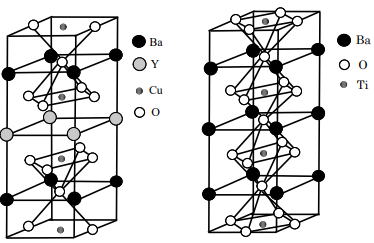
\includegraphics[width=\columnwidth]{kesshoukouzou.png}
          \caption{$\ce{YBa2Cu3O7}$と$\ce{BaTiO3}$の結晶構造}
          \label{fig:kesshoukouzou}
        \end{figure}
      \end{minipage}
    \subsection*{超電導の原理}
      超電導は, ある温度$T_C$以下で物質が電気抵抗を失う現象である. 
      今回扱ったYBCOは, $T_C$が液体窒素温度以上であるため, 高温超電導体と呼ばれる. ペロブスカイト酸化物の超電導の原理はまだ完全には解明されていないため, 
      ここでは金属の超電導の原理を述べる. その理論はBCS理論と呼ばれる. 低温状況下において, 分子の振動が小さくなる.
      格子中を電子が移動すると格子が歪み, その歪みが近くの電子を引き寄せ, 抵抗がなくなる.  
    \subsection*{マイスナー効果}
      超電導体は, 永久電流により反磁場を作り出し, 磁束を排除する. これをマイスナー効果と呼ぶ. 
  \section*{実験}
    \subsection*{実験器具}
      \begin{figure}[H]
        \centering
        \begin{minipage}[H]{0.48\textwidth}
          \centering
          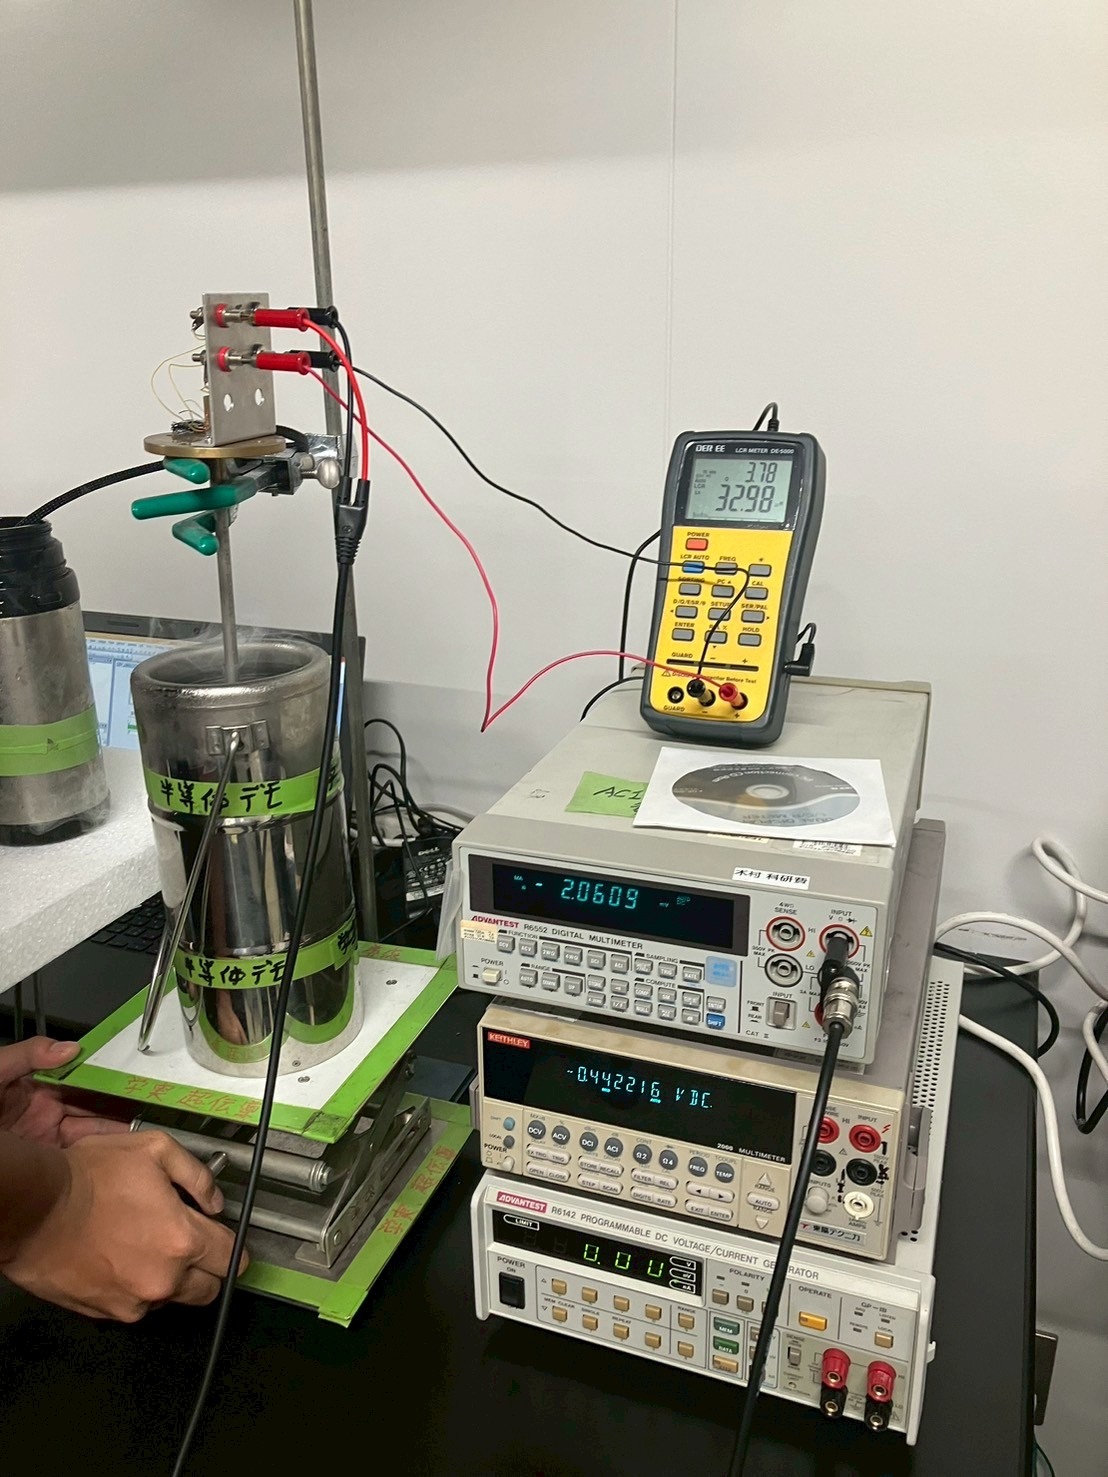
\includegraphics[width=\columnwidth]{jikkenkigu.jpg}
          \caption{実験器具の写真}
          \label{fig:kigu_pic}
        \end{minipage}
        \begin{minipage}[H]{0.48\textwidth}
          \centering
          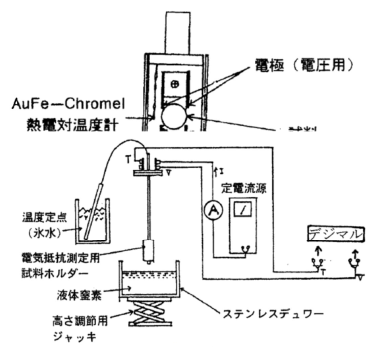
\includegraphics[width=\columnwidth]{jikkenkigu2.png}
          \caption{実験器具の模式図}
          \label{fig:kigu_fig}
        \end{minipage}
      \end{figure}
      写真はインダクタンス測定時のものである. 右の機器は上から, インダクタンス測定器, 熱電対の電圧計, 電圧計, 電流計である.\\
      本実験では温度の測定に熱電対を用いた.
      \subsubsection*{熱電対}
        金属体の両端に温度差があると, 温度差に対応した電位差が生じる.  これをゼーベック効果という. 電位差が温度差に比例するとすると, その比例係数をゼーベック係数と呼ぶ. この係数は金属の種類に依存する.
        したがって, 金属体の両端の電位差を測定すると, 温度差を測定することができる. 電位差を知るためには電圧計の両端に線をつながなければならない.
        しかし, 行きと帰りの同線の金属が同じだと, 電位差がゼロになってしまう. そこで, 異なる金属を用いる. 二つの金属のゼーベック係数がわかっていて, 接点の一端の温度もわかっていれば, もう一端の温度が測定できる.
        今回の測定では, 基準点として氷点(氷水)を用いた. 
        \begin{figure}[H]
          \centering
          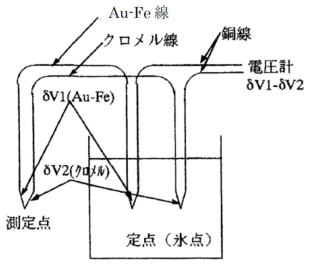
\includegraphics[width=0.6\columnwidth]{netudentui.png}
          \caption{熱電対の接続図}
          \label{fig:netudentui}
        \end{figure}
    \subsection*{試料作製}
      反応式
      \begin{align*}
        \ce{2Y2O3 + 8BaCO3 +12CuO +7O2 -> 4YBa2Cu3O7 + 8CO2}
      \end{align*}
      を用いて, 酸化イットリウム$\ce{Y2O3}$, 炭酸バリウム$\ce{BaCO3}$, 銅$\ce{Cu}$をもちいて高温超電導体YBCO$\ce{YBa2Cu3O7}$を作成する.
      \begin{enumerate}
        \item 原料の秤量\\
              分子量や純度から必要な量を計算し, 原料を秤量した. 
              計算の結果, 実際の量を以下に示す.
              \begin{table}[H]
                \centering
                \begin{tabular}{|c|c|c|}\hline
                  原料 & 計算量 & 実際の量 \\\hline
                  $\ce{Y2O3}$ & 1.774 g & 1.7753 g \\\hline
                  $\ce{BaCO3}$ & 6.3 g & 6.2993 g \\\hline
                  $\ce{CuO}$ & 3.0 g & 2.9989 g \\\hline
                \end{tabular}
                \caption{原料の秤量}
                \label{tab:genryou}
              \end{table}
        \item 原料の混合\\
              秤量した原料を乳鉢に入れ, 粒の大きさが均一になるように, 乳棒でよくすりつぶした. 40分ほどすりつぶした.
        \item 仮焼き\\
              すりつぶした原料をボートにいれ, 電気炉で室温から930 °Cまで8時間かけて加熱し, 930°Cを8時間維持し, 930 °Cから室温まで8時間かけて冷却した.
        \item 粉砕\\
              仮焼きした試料を乳鉢に入れ, 粒が十分小さくなるまで乳棒でよくすりつぶした. 
        \item 加圧成型\\
              すりつぶした試料を加圧して次の三種類の試料を作成した.
              \begin{enumerate}
                \item 直径7 mm, 厚さ0.7 〜2 mmの円盤
                \item 直径7 mm, 高さ10 mmの円柱
                \item 直径30 mm, 厚さ10 mmの円盤
              \end{enumerate}
              (a)は電気抵抗測定用, (b)はインダクタンス測定用, (c)は磁気浮上観察用である.
              加圧はまず$1\mathrm{ton}/0.35\mathrm{\pi cm^2}$の圧力で加圧し, その後$2\mathrm{ton}/0.35\mathrm{\pi cm^2}$の圧力で加圧した.
              \begin{figure}[H]
                \centering
                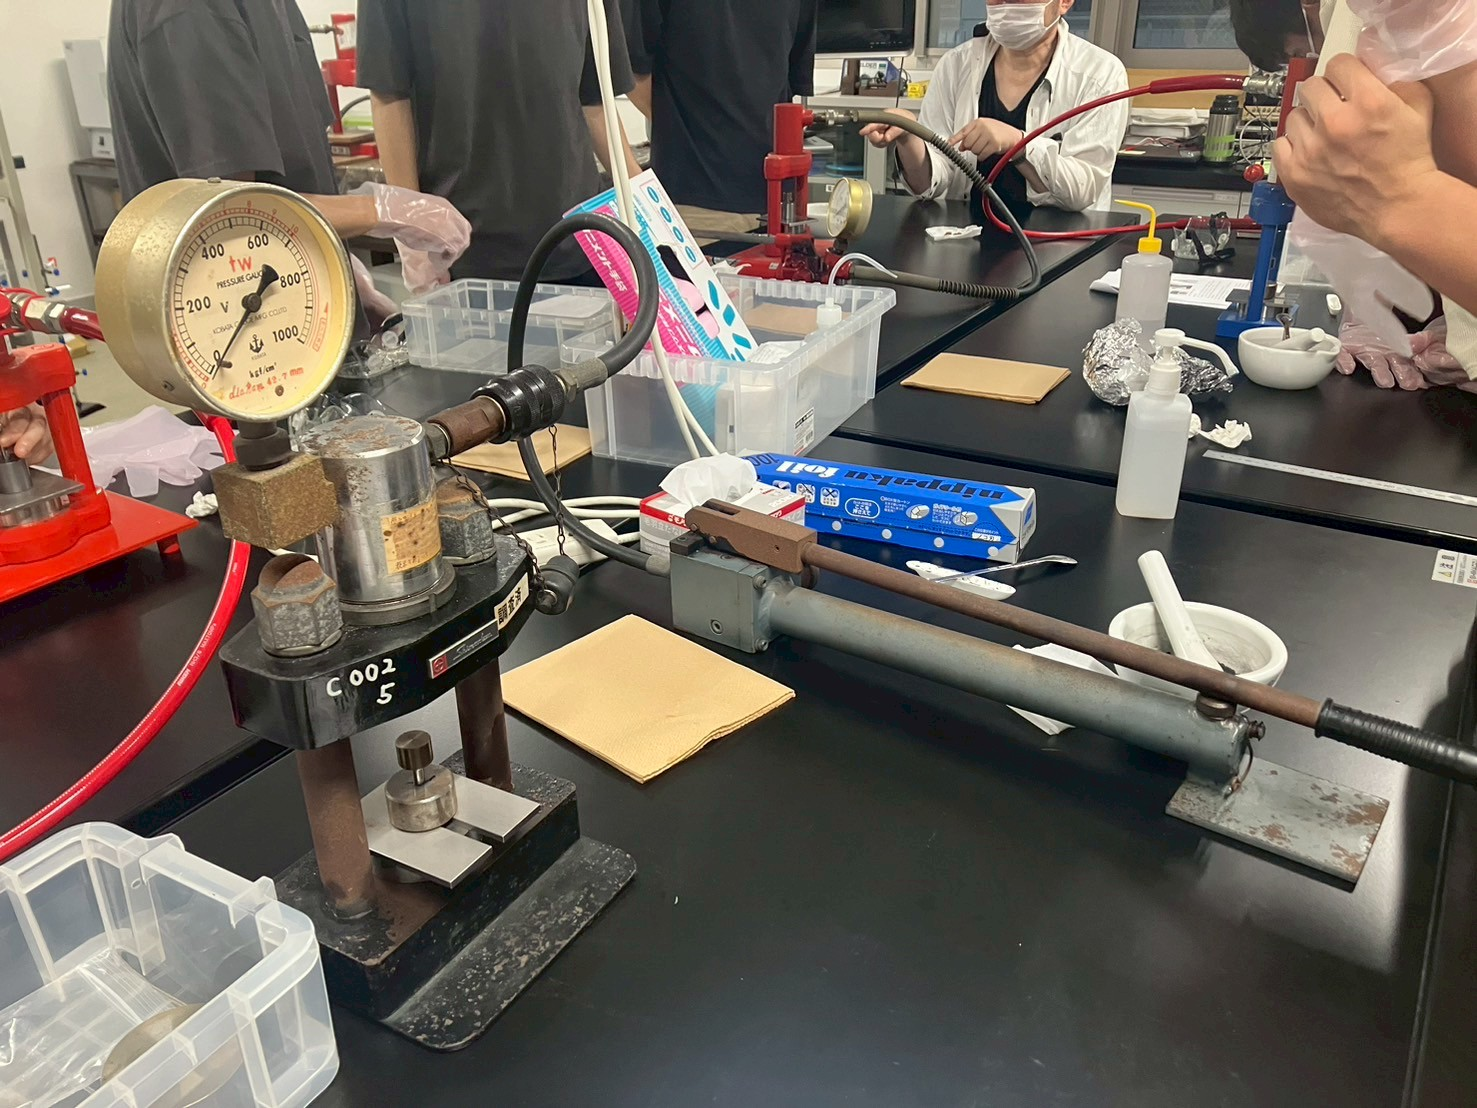
\includegraphics[width=0.4\columnwidth]{kaatu.jpg}
                \caption{加圧成型の様子}
                \label{fig:press}
              \end{figure}
        \item 本焼き\\
              加圧成型した試料をボートに入れ, 仮焼きのときと同様に, 電気炉で室温から930 °Cまで8時間かけて加熱し, 930°Cを8時間維持し, 930 °Cから室温まで8時間かけて冷却した.
              \begin{figure}[H]
                \centering
                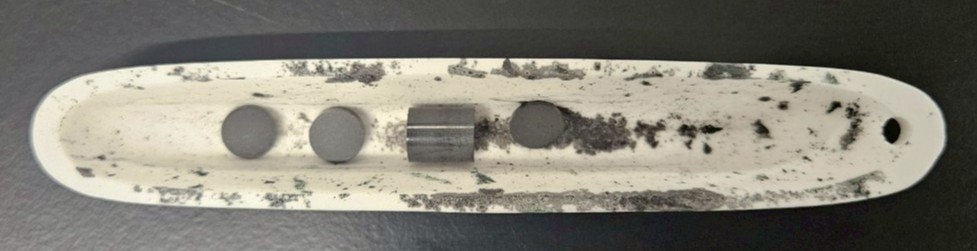
\includegraphics[width=0.4\columnwidth]{kansei.jpg}
                \caption{完成後の試料}
                \label{fig:kansei}
              \end{figure}
      \end{enumerate}
    \subsection*{測定手順}
    \subsubsection*{電気抵抗測定}
      四端子法を用いて, 電気抵抗を測定した.
      \begin{enumerate}
        \item 試料をホルダーにセットし, ねじを締めて端子を試料に密着させ, 電圧端子や電流端子間の抵抗を測定し, 数\Omega 程度であることを確認した.
        \item タンブラーに水と氷を入れたものを温度定点として用意し, 熱電対の一端を入れた. 
        \item \cref{fig:kigu_fig}のように配線した. 
        \item 電流を増やしていった. 具体的には1 mAから始め, 10 mAまで1 mA刻みで増やし, 100 mAまで10 mA刻みで増やした. 電圧が電流に比例すること, つまりオームに法則を確かめた. 
        \item 液体窒素をステンレスデュワーに入れ, プログラムを動かしながらジャッキを操作して試料を液面に近づけていき, 試料全体が液体窒素に浸るようにした. こうして降温過程を記録した.
        \item プログラムを切り替えたのち, ジャッキ操作によって試料を液体窒素から取り出していき, 十分温まるまで昇温過程を記録した.
        \item 試料の厚みを測定した.
      \end{enumerate}
    \subsection*{インダクタンス測定}
      作成した円柱型の試料に銅線を巻き付け, インダクタンスを測定した.
      \begin{figure}
        \centering
        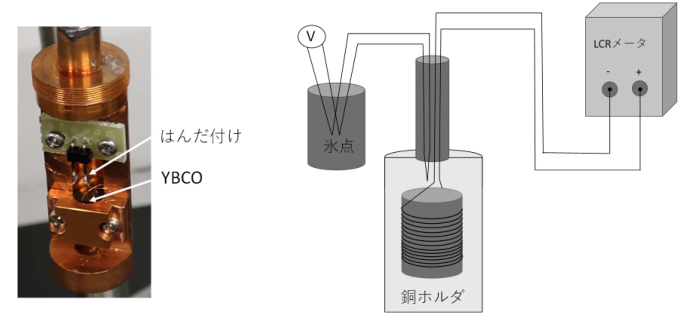
\includegraphics[width=0.6\columnwidth]{Lsokutei.png}
        \caption{(左)銅ホルダの写真 (右)インダクタンス測定の模式図}
        \label{fig:inductor}
      \end{figure}
      \begin{enumerate}
        \item 円柱ペレットにカプトンテープを巻き, 銅線を84回巻き付けたのち,カプトンテープを外から巻きつけた. コイルの長さを測定した.
        \item 巻いたペレットを\cref{fig:inductor}のように銅ホルダにねじで固定し, 銅線をピンヘッダにはんだ付けした. 
        \item \cref{fig:kigu_fig}のように配線し, LCRメータを10 kHzに設定した.
        \item 抵抗測定のときと同様に, 降温, 昇温のときをそれぞれ記録した.
      \end{enumerate}
    \subsection*{磁気浮上観察}
      作成した円盤型の試料を液体窒素に浸し, 磁気浮上を観察した.
      \begin{enumerate}
        \item 円盤ペレットを液体窒素に浸した.
        \item ペレットの上に磁石を置き, ペレットが浮くかどうか観察した.
      \end{enumerate}
  \section*{結果}
    \subsection*{電気抵抗測定}
      \begin{figure}[H]
        \centering
        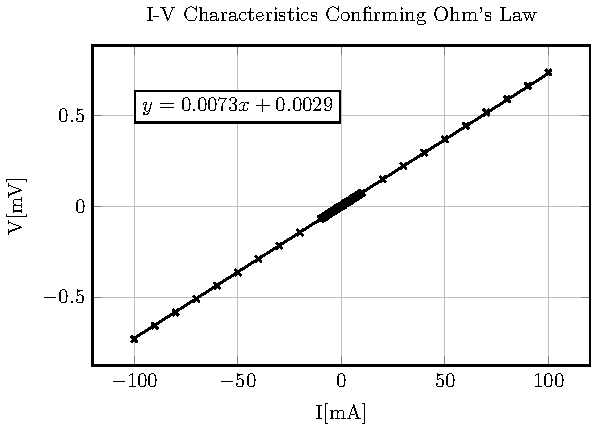
\includegraphics[width=0.6\columnwidth]{solid_graph1.pdf}
        \caption{試料のオームの法則の確認}
        \label{fig:ohm}
      \end{figure}
      \cref{fig:ohm}に示すように, 電流と電圧の関係は直線的であり, オームの法則が成り立つことを確認した.
      \begin{minipage}[H]{0.48\textwidth}
        \centering
        \begin{figure}[H]
          \centering
          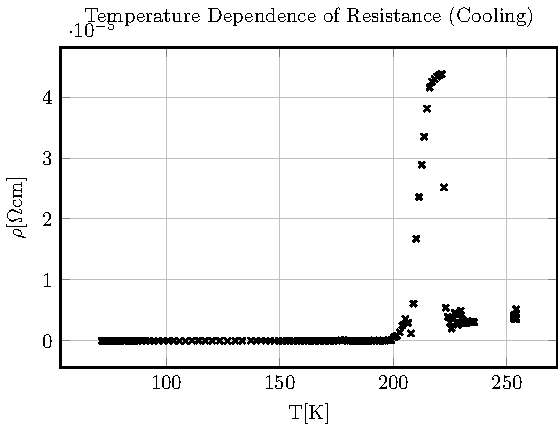
\includegraphics[width=\columnwidth]{solid_graph2.pdf}
          \caption{電気抵抗の温度依存性(降温過程)}
          \label{fig:resistance_cooling}
        \end{figure}
      \end{minipage}
      \begin{minipage}[H]{0.48\textwidth}
        \centering
        \begin{figure}[H]
          \centering
          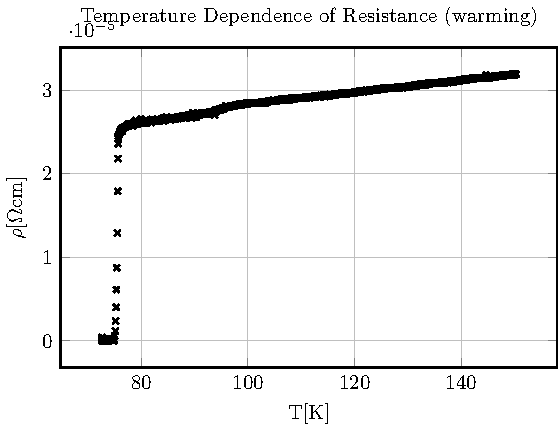
\includegraphics[width=\columnwidth]{solid_graph3.pdf}
          \caption{電気抵抗の温度依存性(昇温過程)}
          \label{fig:resistance_warming}
        \end{figure}
      \end{minipage}
      \cref{fig:resistance_cooling}と\cref{fig:resistance_warming}に示すように, 降温過程では有意なデータは得られなかった. これは, 試料が接点にきちんと接していなかったことが原因と考えられる.
      昇温過程では低温側で抵抗がほぼゼロになり, 温度を上げていくと急激に増加し, その後徐々に増加していく様子が観察された.
    \subsection*{インダクタンス測定}
      \begin{minipage}[H]{0.48\textwidth}
        \centering
        \begin{figure}[H]
          \centering
          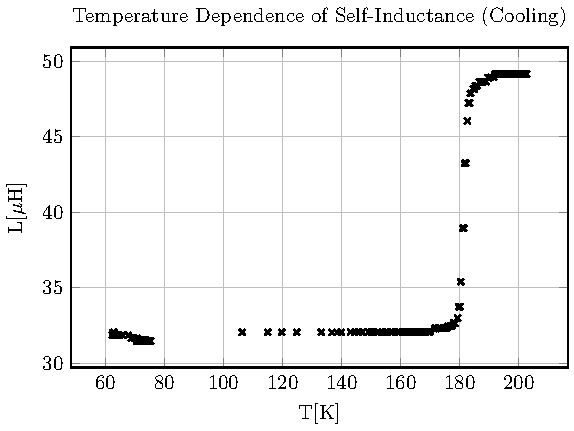
\includegraphics[width=\columnwidth]{solid_graph4.pdf}
          \caption{インダクタンスの温度依存性(降温過程)}
          \label{fig:inductance_cooling}
        \end{figure}
      \end{minipage}
      \begin{minipage}[H]{0.48\textwidth}
        \centering
        \begin{figure}[H]
          \centering
          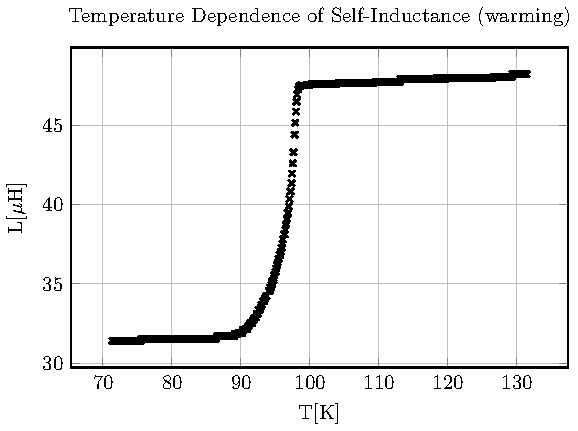
\includegraphics[width=\columnwidth]{solid_graph5.pdf}
          \caption{インダクタンスの温度依存性(昇温過程)}
          \label{fig:inductance_warming}
        \end{figure}
      \end{minipage}
      \cref{fig:inductance_cooling}と\cref{fig:inductance_warming}に示すように, 降温過程では遷移温度がかなり高くなった. また, 80-100Kのデータが不具合によって消えてしまった. 昇温かていでは, 低温でインダクタンスが低く, 温度が上がるにつれてインダクタンスが急激に上昇し, その後徐々に上昇した.
    \subsection*{磁気浮上観察}
      \begin{figure}[H]
        \centering
        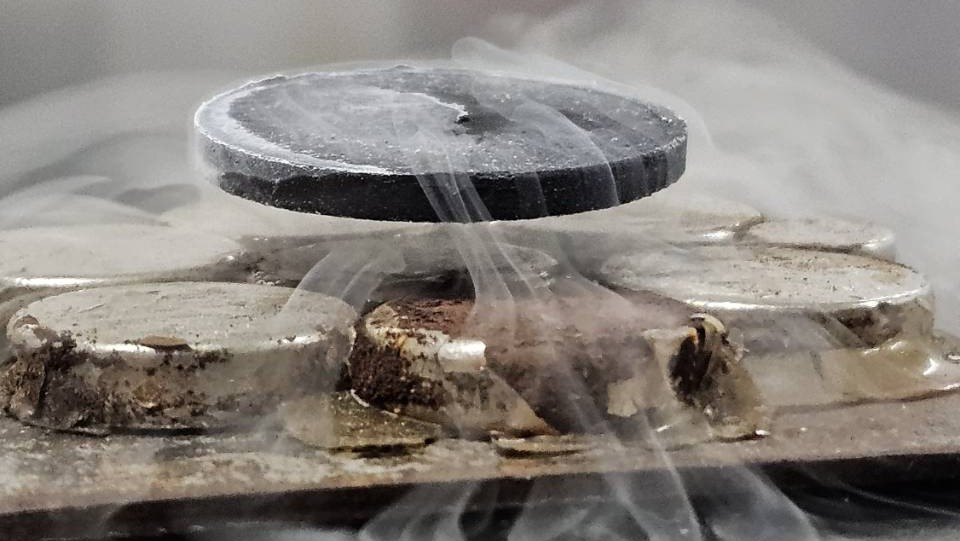
\includegraphics[width=0.6\columnwidth]{79001.jpg}
        \caption{磁気浮上の様子}
        \label{fig:levitation}
      \end{figure}
      \cref{fig:levitation}に示すように, 冷却した円盤型の試料を磁石の上に置くと, 試料が浮上した.
  \section*{課題}
    \subsection*{設問1}
      $\ce{2Y2O3 + 8BaCO3 +12CuO +7O2 -> 4YBa2Cu3O7 + 8CO2}$
      計算結果は以下のようになった.
      \begin{table}[H]
        \centering
        \begin{tabular}{|c|c|}\hline
        原料 & 計算量 \\\hline
        $\ce{Y2O3}$ & 1.774 g \\\hline
        $\ce{BaCO3}$ & 6.3 g \\\hline
        $\ce{CuO}$ & 3.0 g \\\hline
        \end{tabular}
      \end{table}
    \subsection*{設問2}
      計算した密度は3.116 g/cm$^3$であった. また計算結果は6.36 g/cm$^3$であった.
    \subsection*{設問3}
      \begin{enumerate}
        \item 四端子法では, $R=\frac{R_{sample}I_2}{I_1+I_2}$となり, 二端子法では$R=2R_{contact}+2R_{lead}+R_{sample}$となる.
        \item 電圧計の抵抗は, なるべく低い方がよい. その理由は電圧計の抵抗が低いと試料に流れる電流と電流計の値が異なってしまうためである. 四端子法では, 試料と導線の接触抵抗を無視できることが利点である.
        \item 四端子法は接触抵抗や銅線の抵抗の影響を受けず, 二端子法はそれらを無視できるという利点がある.
      \end{enumerate}
    \subsection*{設問4}
      \begin{enumerate}
        \item 21.54\mu Fとなった.
        \item 上で描いた
        \item 透磁率が0にならない理由としては, 超伝導体と銅線の間にすきまがあったこと, 超伝導体の内部に超電導でない点があったことなどから磁束をとおしてしまったからだと考えられる.
      \end{enumerate}
  \section*{考察}
  $T_C^{ON}=75.5$ K, $T_C^{mid}=75.16$ K, $T_C^{0}=75.02$ Kとなった. 液体窒素より温度が低く出た原因として, 熱電対の金属の変容や, 熱電対と試料の比熱の差により温度が違った可能性などが考えられる. また, 降温過程で遷移温度が高くなった原因として, 熱電対が試料より上にあったことにより, 試料は液体窒素に触れているのに, 熱電対はまだ液体窒素に触れていないといった可能性が考えられる.
  密度がかなり違ったのは, 空隙があることや, 圧縮が不十分だったことなどが考えられる.
  \section*{まとめ}
  今回の実験では, 高温超伝導体YBCOを作成し, 電気抵抗, インダクタンス, 磁気浮上を観察することができた.
  \section*{参考文献}
  固体物性テキスト
\end{document}